\scanpage{14}
\figure{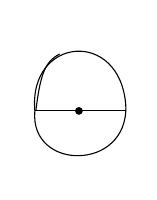
\begin{tikzpicture}[scale=.7]
\draw (0,0) .. controls (-.12,1.35) and (1.55,1.5) .. (1.65,.1) .. controls (1.7,-1.1) and (-.1,-1.1) .. (0,0);
\draw (0,0)--(1.65,0);\fill (.8,0) circle (2pt);
\draw (.02,.02) .. controls (.1,.65) and (.18,.9) .. (.45,1.03);
\end{tikzpicture}}
NB
\[
\mu_n=\operatorname{Ker}(G_m\xrightarrow{n}G_m)
\]
\[
\mu_n(X')=\deleted{\operatorname{Ker}}{}_n\Gamma(X',\mathcal O_{X'})^*
\]
\margin{$\mu_n$ fini plat sur $X$}

Si $n$ premier aux car de $X$, $\mu_{nX}$ est \uline{étale} sur $X$ loc. isom. (pour top. étale) à $\mathbf Z/n\mathbf Z$. Il n'faut surtout pas les confondre. Les $\mu_{nX}^{\otimes d}$ $(d\in\mathbf Z)$ sont donc définis, et sont \inserted{loc} isomorphes à $(\mathbf Z/n\mathbf Z)_X$ [le choix d'une section primitive de $\mu_n$ définit un isom $\mu_{nX}^{\otimes d}\simeq(\mathbf Z/n\mathbf Z)_X$, multiplier cette section par $\lambda\in\mathbf Z/n\mathbf Z$ multiplie l'isom précédent par $\lambda^d$ ...]. \uline{Dém} presque immédiate par th. de changement de base......

\uline{Pb} \fbox{Pureté ``absolue''} \unsure{avec|sans} hypothèse de \unsure{lissité} remplacée par hyp. de régularité. OK. \inserted{pour bons premiers} en égales car. quand on dispose de la résolution des singularités (Artin).

Il y a aussi un th de pureté relatif sur une base quelconque ....

\deleted{13)}

Extension aux div. à croisements normaux....

\deleted{13) \uline{Les} $R^i_!f_*(F)$.

Morphismes \unsure{compactifiables} $f:X\to Y$.
\unsure{On factorise en} $\unsure{X'}\xrightarrow{i}\overline X\ \unsure{\perp}\ Y$, où $i$ : \unsure{imm.}}
\mspage{13}
